\documentclass{article}

% Pakkar
\usepackage[utf8]{inputenc} % UTF-8 kóðun
\usepackage[T1]{fontenc}    % Leturkóðun fyrir íslenska stafi
\usepackage{graphicx}       % Fyrir myndir
\usepackage{listings}       % Fyrir kóðalista
\usepackage{xcolor}         % Fyrir sérsniðna liti
\usepackage{minted}         % Fyrir syntax highlighting
\usepackage{hyperref}       % Fyrir krækjur

% Skilgreina sérsniðna liti fyrir syntax highlighting
\definecolor{keywordcolor}{rgb}{0,0,0.8}
\definecolor{commentcolor}{rgb}{0,0.5,0}
\definecolor{stringcolor}{rgb}{0.58,0,0.82}

% Breyta myndamerki yfir á íslensku (ef óskað)
\renewcommand{\figurename}{}

\title{}
\author{}
\date{} % No date

% Kóðalista stillingar (Listings)
\lstset{
  language=[x86masm]Assembler, 
  basicstyle=\footnotesize\ttfamily, 
  numbers=left, 
  numberstyle=\tiny, 
  stepnumber=1, 
  numbersep=5pt, 
  backgroundcolor=\color{white}, 
  showspaces=false, 
  showstringspaces=false, 
  showtabs=false, 
  tabsize=2, 
  captionpos=b, 
  breaklines=true, 
  breakatwhitespace=false, 
  keywordstyle=\color{keywordcolor}\bfseries,
  commentstyle=\color{commentcolor}\itshape, 
  stringstyle=\color{stringcolor}, 
  frame=single, 
  framerule=0.5pt,
  framesep=2mm,
  escapeinside={\%*}{*)},
  morekeywords={MOV,ADD,SUB,MUL,DIV,PUSH,POP,CALL,RET,JMP,JE,JNE,JG,JL,JGE,JLE},
}

\begin{document}

\maketitle

\section{MIC MVP Release v2.0.0-beta}

\subsection{Introduction}
This is a MVP release of a brand new version of Map in Color (MIC) v2.0.0-beta,
a tool for creating choropleth maps to visualize data---whether for scientific 
purposes or simply to see the world from a new perspective through data.

With the new version, the application includes more complexity and a sharing platform 
where data can be shared between users. Instead of manually selecting and defining 
states from select inputs (as seen in v1), you prepare a CSV file locally with all 
the data for the map, ensuring simplicity.

This MVP release features:
\begin{itemize}
  \item A set of three maps (World Map, United States, and Europe) -- with 
    more to be added over time.
  \item The ability to instantly generate data ranges with ease (either 
    suggested or manually defined).
  \item A sharing platform with tags for potential future data collection 
    across diverse subjects, browsable via an \emph{explore} page.
  \item Public or private map settings for each user’s preference.
  \item User profiles that allow personal info, stars, 
    and comments on maps.
\end{itemize}

\section{Quick Start (For Users)}

\begin{enumerate}
  \item Sign Up

  Go to mapincolor.com and fill out the sign-up form. After a successful 
  registration, you will be taken to your Dashboard.

  \item Create Your First Map
  \begin{itemize}
  \item Use the sidebar or header to click "Create New Map."
  \item Select which map template you want (World, USA, or Europe) in the pop-up.
  \item Click "Create". You will be taken to the 
      Data Integration page.
  \end{itemize}

  \item Data Integration
  \begin{itemize}
  \item Prepare your CSV file (see details below) and upload it.
  \item Define data ranges (either by manual input or by generating suggested ranges).
  \item Adjust colors and theme settings (ocean color, unassigned states, etc.).
  \item Fill out map details (title, description, tags, references).
  \end{itemize}

  \item Save \& Share
  \begin{itemize}
  \item Choose public or private for your map.
  \item Click "Save Map".
  \item You can now view or edit your map from your collection, explore other 
      maps, star, and comment.
  \end{itemize}
\end{enumerate}

\section{How to Create and Edit Maps}

When you navigate to the Data Integration page, have your CSV file ready. 
It must contain exactly two columns:

\begin{enumerate}
  \item Country/State Name
  \item Value
\end{enumerate}

\noindent
No values can be empty.

\subsubsection*{Example CSV}

\begin{minted}{text}
Country/State Name,Value
State1,Value1
State2,Value2
...
\end{minted}

If your CSV is successfully uploaded, you may see summary statistics about the file.

\begin{figure}[h!]
  \centering
  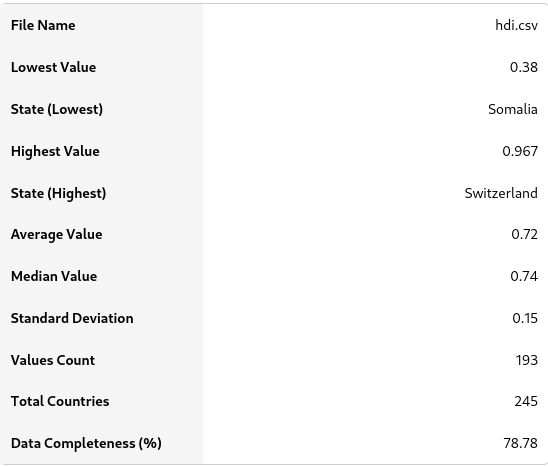
\includegraphics[width=0.7\textwidth]{stats.png}
  \caption{Statistics Example}
\end{figure}

\subsection{Error Handling}

If a state name isn’t recognized or the file is invalid, you’ll see an 
error log showing the line number and the issue:

\begin{figure}[h!]
  \centering
  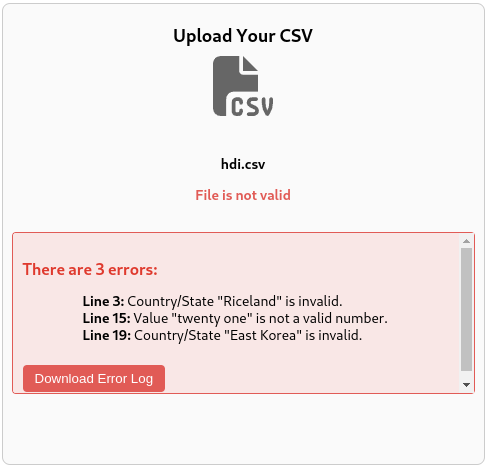
\includegraphics[width=0.7\textwidth]{error.png}
  \caption{Error Log Example}
\end{figure}

Fix any errors and re-upload until you see a success message:

\begin{figure}[h!]
  \centering
  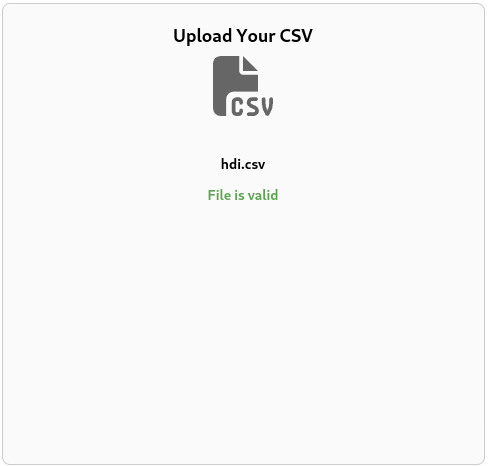
\includegraphics[width=0.7\textwidth]{valid.png}
  \caption{Valid CSV Example}
\end{figure}


\section{Defining Ranges}

\subsection{Suggested vs. Manual}

\begin{itemize}
  \item Manual: Type in your lower and upper bounds for each range.
  \item Auto-Generate: Specify how many ranges you want and click
    "Suggest range".
\end{itemize}

\noindent
For example, you can press certain buttons to define or suggest ranges:

\begin{figure}[h!]
  \centering
  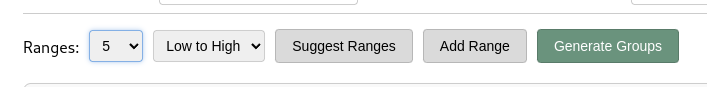
\includegraphics[width=0.7\textwidth]{range_buttons.png}
  \caption{Range Buttons Example}
\end{figure}

\subsection{Name \& Coloring}

Name each range (e.g., “Low,” “Medium,” “High,” etc.). Choose individual colors or 
use a provided color palette. Then click "Generate Groups" to 
update the map with the new ranges.

\section{Theme \& Final Settings}

You can adjust map details: ocean color, unassigned color, etc. 
For example:

\begin{figure}[h!]
  \centering
  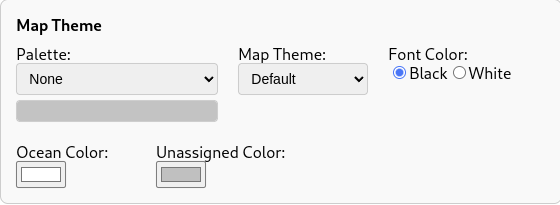
\includegraphics[width=0.7\textwidth]{map_theme.png}
  \caption{Theme Settings Example}
\end{figure}

Then fill out title, description, tags, 
references, and decide if the map is private or public:

\begin{figure}[h!]
  \centering
  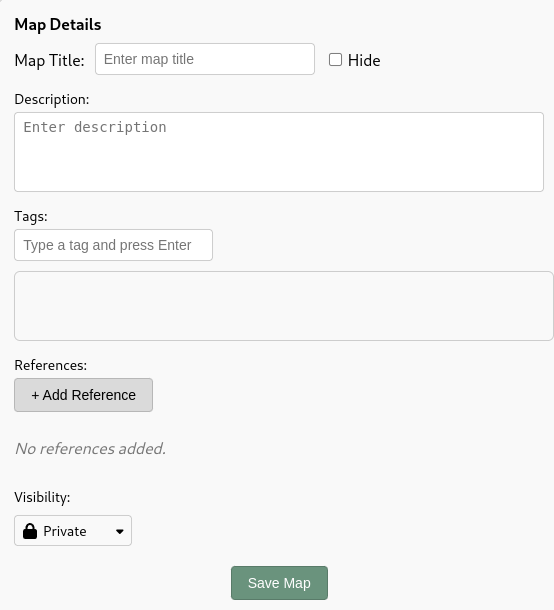
\includegraphics[width=0.7\textwidth]{map_details.png}
  \caption{Map Details Example}
\end{figure}

Finally, press "Save Map". The map is now in your collection, and you can 
edit it anytime.

Once saved, you can star or comment on maps, explore other 
users’ public maps, and further customize your own.

\end{document}
